\section{Benchmarking the~AWBS nonlocal transport model}
\label{sec:BenchmarkingAWBS}
Having shown several encouraging properties of the~AWBS transport 
equation defined by \eqref{eq:AWBS_model} under local diffusive conditions
in \secref{sec:DiffusiveKinetics}, this section focuses on analyzing 
its behavior under nonlocal plasma conditions, extensively investigated 
in numerous publications 
\cite{Malone_1975_15, Colombant_PoP2005, Bell_1981_83, LMV_1983_7, Brantov_Nonlocal_electron_transport_1998, schurtz2000, Sorbo_2015}.
A~variety of tests suitable for benchmarking the~nonlocal electron 
transport models have been published 
\cite{Epperlein_PoFB1991, marocchino2013, Sorbo_2015, 
Sorbo_2016, Sherlock_PoP2017, Brodrick_PoP2017}, we focus on 
conditions relevant to inertial confinement fusion plasmas generated by lasers.

We show results of our implementation of the~AP1 nonlocal transport model 
presented in \secref{sec:AWBSnonlocal} benchmarked against simulation results 
provided by a~rather complete set of kinetic models with varying complexity. 
The~most reliable models represents a~collisional Particle-In-Cell
code Calder \cite{Lefebvre_NF2003, Perez_PoP2012} resolving 
the~plasma frequency time scale, and a~standard VFP codes
Aladin and Impact \cite{Kingham_JCP2004}.
In addition, we compare the~SNB nonlocal transport model \cite{Schurtz_2000} 
used in hydrodynamic codes. 
That is a~first time when a~collisional PIC code is used
for benchmarking of nonlocal electron transport models. 

%%% CEA contribution starts
\textbf{Calder PIC code}

The~particle evolution in the~phase-space, including small angle 
binary collisions, is described with 
the~Maxwell equations \eqref{eq:Faraday}, \eqref{eq:Ampere}
%\begin{eqnarray}
%&&\nabla\cdot \mathbf{E}=\sum_\alpha \frac{q_\alpha}{\varepsilon_0} n_{\alpha},\\
%&&\nabla\cdot \mathbf{B}=0,\\
%&&\nabla\vect{\times} \mathbf{E}+\frac{\partial \mathbf{B}}{\partial t}=0,\\
%&&\nabla\vect{\times} \mathbf{B}-\mu_0\varepsilon_0\frac{\partial \mathbf{E}}{\partial t}=\mu_0\sum_\alpha\mathbf{j}_{\alpha},\label{maxw}
%\end{eqnarray}
coupled with the~ion and electron Vlasov equations with 
the~Landau-Beliaev-Budker collisions integral (LBB)
\cite{Landau_1936, Beliaev_SPD1956} 
\begin{multline}
\frac{\partial f_\alpha}{\partial t}+\mathbf{v}\cdot\nabla_{\mathbf{x}}f_\alpha+q_\alpha\left(\mathbf{E}+\mathbf{v}\vect{\times}\mathbf{B}\right)\nabla_{\mathbf{p}}f_\alpha =
\\
C_{LBB}(f_\alpha,f_\alpha)+\sum_\beta C_{LBB}(f_\alpha,f_\beta)
.
\end{multline}
The LBB collision integral takes the~form
\begin{multline}
C_{LBB}(f_\alpha,f_\beta)=
\\
-\frac{\partial}{\partial \mathbf{p}}\cdot\frac{\Gamma_{\alpha\beta}}{2}\left[\int \mathbf{U}(\mathbf{p},\mathbf{p}^\prime)\cdot(f_\alpha\nabla_{\mathbf{p}^\prime}f_\beta^\prime-f_\beta^\prime\nabla_{\mathbf{p}}f_\alpha)\right]d^3\mathbf{p}^\prime
,
\label{eq:LBB_model}
\end{multline}
where its relativistic kernel reads
$\mathbf{U}(\mathbf{p},\mathbf{p}^\prime)=\frac{r^2/\gamma\gamma^\prime}{(r^2-1)^{3/2}}$ 
$\left[(r^2-1)\mathbf{I}-\mathbf{p}\otimes\mathbf{p}-\mathbf{p}^\prime\otimes\mathbf{p}^\prime+r(\mathbf{p}\otimes\mathbf{p}^\prime+\mathbf{p}^\prime\otimes\mathbf{p})\right]$
with $\gamma=\sqrt{1+\mathbf{p}^2}$, $\gamma^\prime=\sqrt{1+\mathbf{p}^{\prime 2}}$ and $r=\gamma\gamma^\prime-\mathbf{p}\cdot\mathbf{p}^\prime$. 
The momemtum $\mathbf{p}_\alpha$ ($\mathbf{p}_\beta$) is normalized to 
$m_\alpha c$ (resp. $m_\beta c$). The~collision operator \eqref{eq:LBB_model} 
tends to \eqref{eq:LFP_model} in the non-relativistic limit.
%described in Appendix~\ref{app:CalderKinetics}. 
%The~latter is the~relativistic version of the~collision operator 
%introduced in \eqref{eq:LFP_model}. 
The aforementioned model is solved in 3D by the PIC code CALDER. 
\cite{Lefebvre_NF2003, Perez_PoP2012}.

\textbf{Impact and Aladin VFP codes}

PIC simulations are extremely expensive as the~collisions require description 
of the~velocity space in 3 dimensions. Yet, a~reduction of dimensions can be 
done by developing the~distribution function in a~Cartesian tensor series, 
equivalent to expansion in the spherical harmonics \cite{Johnston_PR1960}.
%as follows:\textit{CPR comment - Cartesian tensors are the same as spherical harmonics to first order}
%\begin{equation}
%  f(t,\mathbf{x},\vv) = f_0(t,\mathbf{x},\vmag) 
%  + \vn\cdot \vect{f}_1(t,\mathbf{x},\vmag)
%  +\vn\otimes\vn:\matr{f}_2(t,\mathbf{x},\vmag)+... .
%  \label{Pn}
%\end{equation}
%where $v=|\mathbf{v}|$, $\Omega=\mathbf{v}/v$. 
%A P$_n$ model refers to 
%neglecting orders higher than $\matr{f}_n$. 
The~first order form corresponds to the~P1 approximation 
\eqref{eq:P1approximation} and coupled with
%distribution function 
%approximation $f(t,\mathbf{x},\vv)\approx f_0(t,\mathbf{x},\vmag)
%+\vn\cdot \vect{f}_1(t,\mathbf{x},\vmag)$ coupled with 
the~Landau-Fokker-Planck collisional operator 
\eqref{eq:LFP_model} leads to the P$_1$-VFP model 
\cite{Johnston_PR1960, Kingham_JCP2004}:
\begin{eqnarray}
\frac{\partial \fzero}{\partial t}+\frac{\vmag}{3}\nabla \cdot \fone
+\frac{\qe}{3\me\vmag^2}\frac{\partial}{\partial \vmag}(\vmag^2\E\cdot \fone)
&=&
C^0_{ee}(\fzero) ,
 \label{eq:P1f0_Aladin}\\
\frac{\partial \fone}{\partial t}+\vmag\nabla \fzero
+ \frac{\qe\E}{\me}\frac{\partial \fzero}{\partial \vmag}
+\frac{\qe\B}{\me}\vect{\times} \fone 
&=&
- \nuei\fone .
\label{eq:P1f1_Aladin}
\end{eqnarray}
where only the~isotropic part of the~distribution function in 
in the~e-e collision integral \eqref{eq:LFP_model} is used as the~following
\begin{eqnarray} 
C^0_{ee}(\fzero) &=& \frac{\Gamma}{v^2}\frac{\partial}{\partial \vmag}
\left[C(f_0)f_0+D(\fzero)\frac{\partial \fzero}{\partial \vmag}\right] ,
\label{eq:C0_collision_operator}
\\
C(\fzero(\vmag)) &=& 4\pi\int_0^\vmag \fzero(u) u^2 \dI u ,
\nonumber
\\
D(\fzero\vmag)) &=& \frac{4\pi}{\vmag}\int_0^\vmag u^2\int_u^\infty w \fzero(w) 
\dI w \dI u .
\nonumber
\end{eqnarray}

The~codes Impact and Aladin solve the system \eqref{eq:P1f0_Aladin} 
and \eqref{eq:P1f1_Aladin} with the Maxwell equations  
\eqref{eq:Faraday} and \eqref{eq:Ampere} in two spatial dimensions, 
assuming immobile ions.

The~model AP1 uses similar equations as Aladin
and Impact with the~difference, that AP1 describes the~steady-state 
electron distribution function with respect to the~ions,
and is using a~simplified (linear) collision operator inherently
coupled to ions via the~hydrodynamic equations.

%%% CEA contribution ends

\textbf{SNB approach}

Now considered as a~standard nonlocal electron transport models in hydrodynamic 
codes, SNB \cite{Schurtz_2000} represents an efficient P1 method based on
the~velocity dependent form of the~collision BGK operator. It uses EDF 
approximation representing deviation from the~local BGK theory
\begin{equation}
  \tilde{\ft} = 
  \fM + \delta\fzero 
  + \vn\cdot\left(\fone_M + \delta\fone\right) . 
  \label{eq:SNB_approximation}
\end{equation}
%where $\fone_M = - \xi\mfpei\left( \frac{\vmag^2}{2 \vth^2} - 4\right)\fM
%\frac{\nabla \Te}{\Te}$ is obtained from the~diffusive solution 
%\eqref{eq:BGK_approximation} with \eqref{eq:BGK_scaling}.
Equations for the~zero and first angular moments follow from 
the~electron transport equation with scaled collision operator 
\eqref{eq:BGK_scaling}
according to the~SNB approximation \eqref{eq:SNB_approximation} 
(similar to \eqref{eq:AP1f0} and \eqref{eq:AP1f1})
\begin{eqnarray}
  r_B \delta\fzero &=&
  - \frac{\vmag}{3}\nabla\cdot\delta\fone
  - \frac{\vmag}{3}\nabla\cdot\fone_M
  \nonumber\\ 
  &&\xcancel{- \frac{\qe}{\me}\frac{\E}{3}\cdot\left(
  \pdv{\fone_M}{\vmag} + \pdv{\delta\fone}{\vmag} 
  + \frac{2}{\vmag}\left(\fone_M + \delta\fone\right)\right)} , 
  \nonumber \\
  \label{eq:SNBf0}\\
  \frac{\nuei}{\xi}\delta\fone &=& - \vmag\nabla\delta\fzero 
  ~\xcancel{- \frac{\qe}{\me}\E\pdv{\delta\fzero}{\vmag}}
  %- \omegaB\vect{\times} \delta\fone } 
  \nonumber \\
  &&\underbrace{- \frac{\nuei}{\xi}\fone_M - \vmag\nabla\fM
  - \frac{\qe}{\me}\E\pdv{\fM}{\vmag}
  %- \omegaB\vect{\times} \fone_M
  }_{~~~~~~~~~~~~~=~0~defines~\fone_M} 
  %+\frac{\qe\B}{\me c}\vect{\times} \left(\fone_M + \delta\fone\right)
  ,
  \nonumber \\
  \label{eq:SNBf1}
\end{eqnarray}
where the~magnetic field was neglected, the~under-braced part
of \eqref{eq:SNBf1} when $\delta\fzero$ and $\delta \fone$ are zero
defines the~local anisotropic term
%where $\fone_M = \frac{\frac{\nuei^2}{\xi^2} \vect{F}_M 
%+ \omegaB~\omegaB\cdot\vect{F}_M - \frac{\nuei}{\xi}~\omegaB \vect{\times} 
%\vect{F}_M}{\frac{\nuei}{\xi} \left(\omegaB^2 + \frac{\nuei^2}{\xi^2}\right)}$
%, where $\vect{F}_M = -\vmag \left( \frac{\fM}{\ed}\nabla\ed 
%+ \left( \frac{\vmag^2}{2\vth^2} - \frac{3}{2}\right)
%\frac{\fM}{\Te}\nabla\Te - \frac{\qe \fM}{\me\vth^2}\E\right)$.
\begin{equation}
  \fone_M = -\xi\mfpei\fM\left( \frac{\nabla\ed}{\ed} 
+ \left( \frac{\vmag^2}{2\vth^2} - \frac{3}{2}\right)
\frac{\nabla\Te}{\Te} - \frac{\qe\E}{\me\vth^2}\right) ,
  \label{eq:f1M}
\end{equation}
%One should notice, that the~local
%EDF contribution cancels out in \eqref{eq:SNBf1} when the~electric field 
%adjusts to the~local Lorentz electric field \eqref{app_eq:BGK_Efield}. 
and the~efficiency of SNB resides in omitting the~electric field 
effect (crossed out terms in \eqref{eq:SNBf0} and \eqref{eq:SNBf1}), which
leads to a~simple diffusion equation for the~correction to the~isotropic 
part of the~distribution function
\begin{equation}
  \frac{1}{\mfpe^{SNB}}\delta\fzero 
  - \nabla\cdot\frac{\mfpei^{SNB}}{3}\nabla\delta\fzero =
  \nabla\cdot\frac{\xi\mfpei}{3}\fM\frac{\nabla \Te}{\Te}
  ,
  \label{eq:SNB_model}
\end{equation}
where $\frac{1}{\mfpei^{SNB}} = 
\frac{\nuei}{\xi\vmag} + \frac{|\qe\E|}{\frac{1}{2}\me\vmag^2}$ 
and $\mfpe^{SNB} = \frac{\vmag}{r_B \nue}$, and the~source term based on 
$\fone_M$ simplifies by avoiding the~electric field effect, density gradient 
and the~$\vmag$-dependent bracket in \eqref{eq:f1M}. The~missing
effect of $\E$ in \eqref{eq:SNB_model} is accounted for by 
an~isotropic scattering in definition of $\mfpei^{SNB}$ \cite{Schurtz_2000}.
Consequently, the~effect of the~electric field in SNB
is accounted for only via $\fone_M$, where the~electric field is
fixed to $\E_L$. 
%A~self consistent zero current condition 
%$\vect{j} = \qe \int \vmag (\fone_M + \delta\fone)~\dI\tilde{\vmag} = 0$ then
%defines the~actual value of the~electric field from \eqref{eq:SNBf1} as
%\begin{equation}
% \E = -\frac{\int \frac{\xi\vmag^2}{\nuei}\nabla
% \left(\fM + \delta\fzero\right)~\dI\tilde{\vmag}}
% {\int \frac{\xi\vmag}{\nuei}\frac{\qe}{\me}\pdv{\fM}{\vmag}
% ~\dI\tilde{\vmag} } 
% = \E_L - \frac{\int \frac{\vmag^2}{\nuei}\nabla
% \delta\fzero~\dI\tilde{\vmag}}
% {\frac{\qe}{\me}\int \frac{\vmag}{\nuei}\pdv{\fM}{\vmag}
% ~\dI\tilde{\vmag} } ,
% \label{eq:SNB_E} 
%\end{equation}

As shown previously, the~BGK collision operator \eqref{eq:BGK_scaling}
provides one free parameter $\zeta$.
We propose to use $\zeta = 2$ giving $r_B(\Zbar\gg1) = 2$ which agrees 
with $r=2$ in SNB formulation proposed in \cite{Brodrick_PoP2017} 
for the~case of ICF relevant plasma. We also have $r_B(\Zbar = 1) = 1.677$,
which means that our pure kinetic derivation of SNB varies just slightly
from a~constant value $r_B=2$ \cite{Brodrick_PoP2017}, yet it provides 
slightly better results. The~explicit form of the~anisotropic 
part of EDF then reads $\fone = \fone_M - \mfpei^{SNB}\nabla\delta\fzero$.

\begin{figure*}[htb]
  \begin{center}
    \begin{tabular}{cc}
      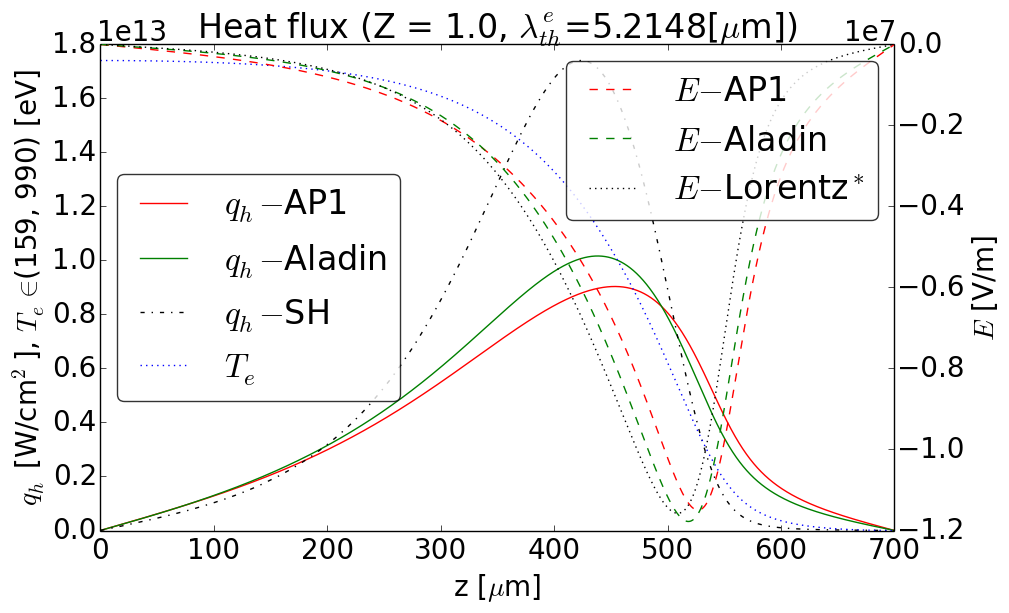
\includegraphics[width=\figscale\textwidth]{../VFPdata/C7_Aladin_case5_heatflux.png} 
	  &
      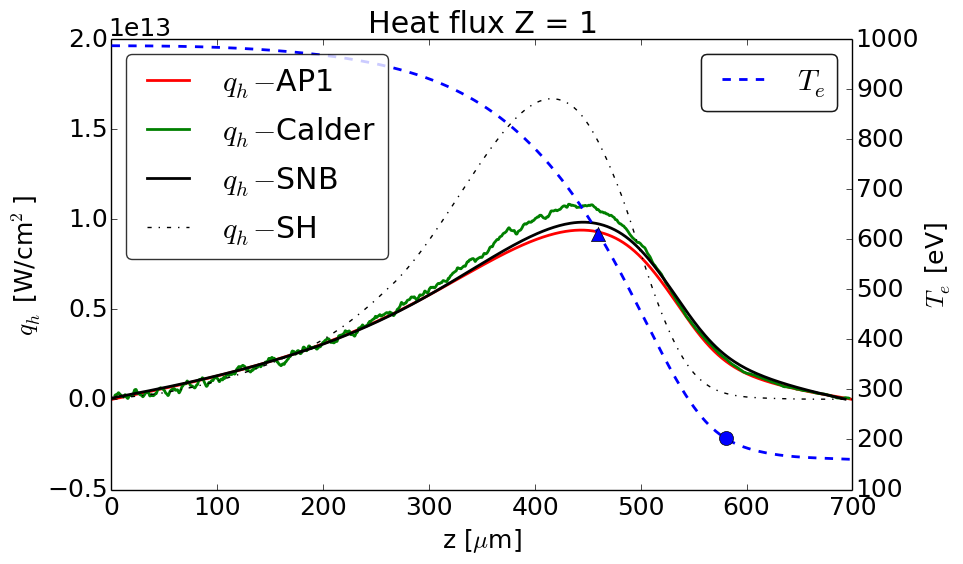
\includegraphics[width=\figscale\textwidth]{../VFPdata/C7_Calder_case5_heatflux.png} 
	  \\ 
      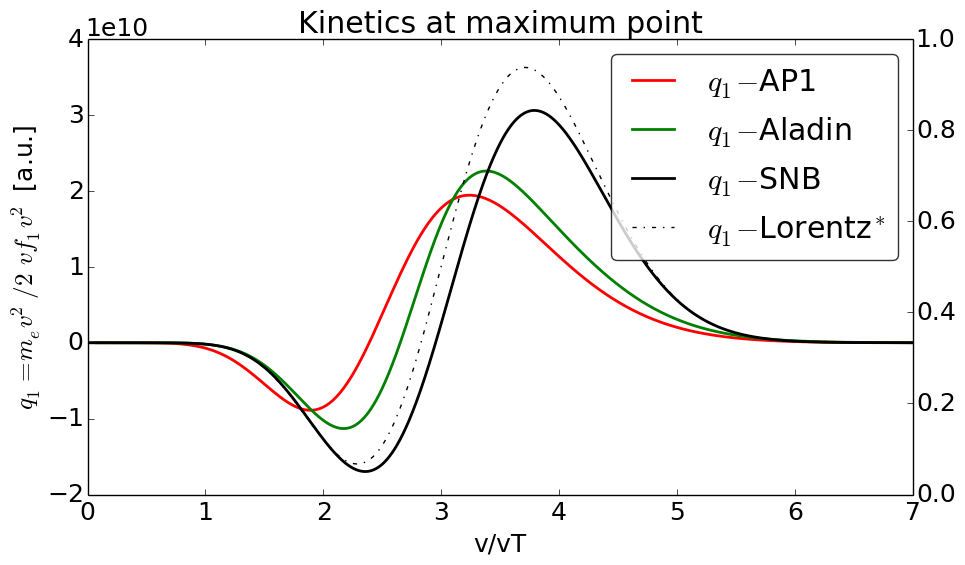
\includegraphics[width=\figscale\textwidth]{../VFPdata/C7_Aladin_case5_kinetics.png} 
	  &
      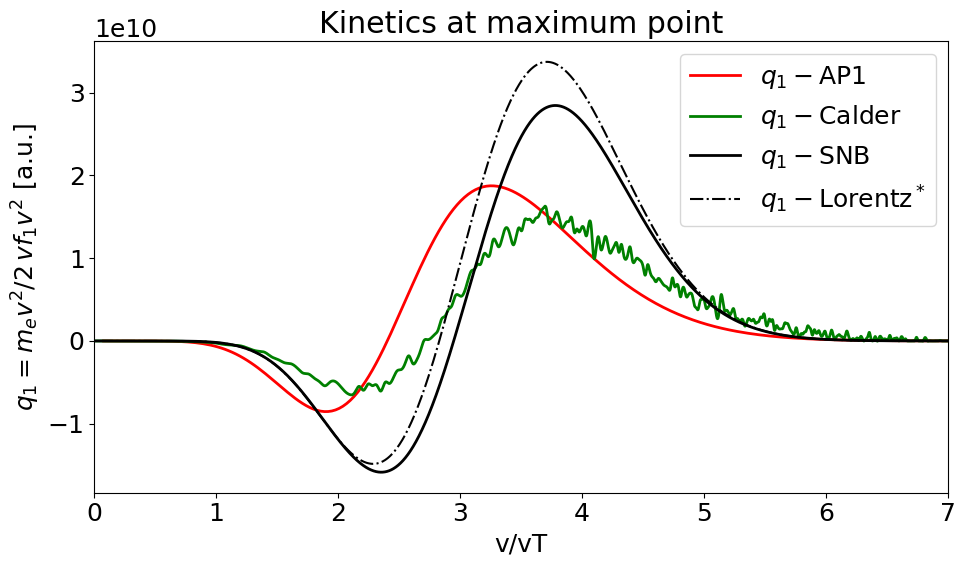
\includegraphics[width=\figscale\textwidth]{../VFPdata/C7_Calder_case5_kinetics.png} 
	  \\
	  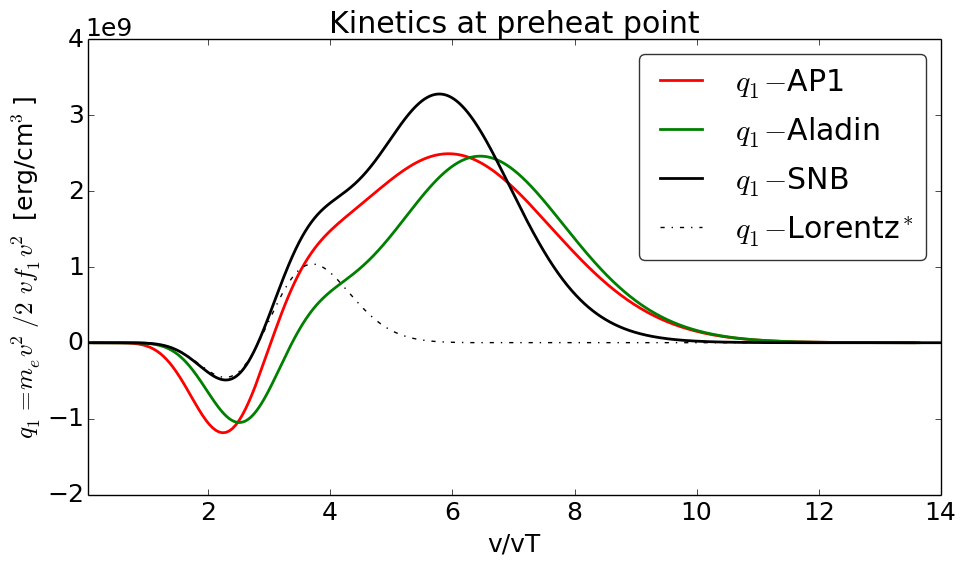
\includegraphics[width=\figscale\textwidth]{../VFPdata/C7_Aladin_case5_nonlocal_kinetics.png} 
      &
      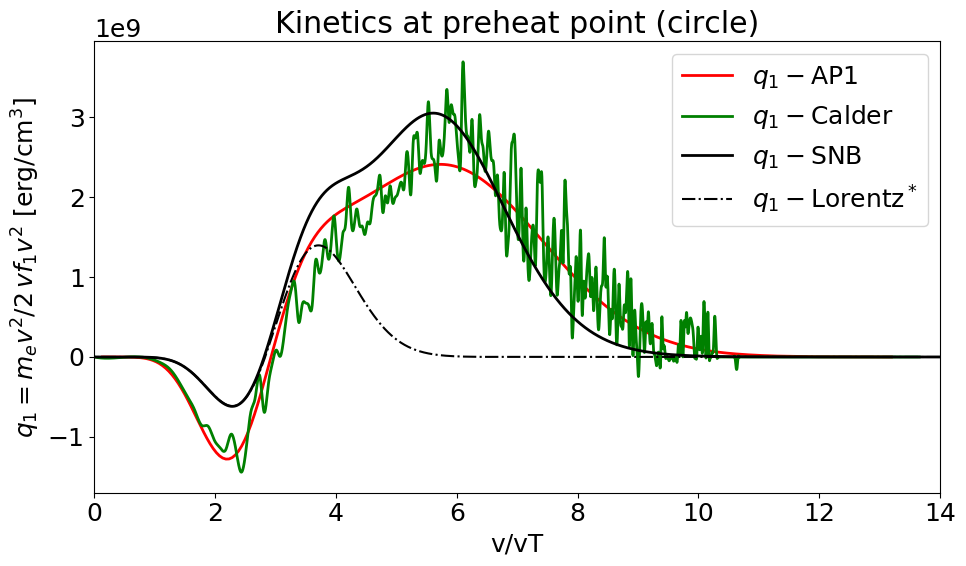
\includegraphics[width=\figscale\textwidth]{../VFPdata/C7_Calder_case5_nonlocal_kinetics.png}
	\end{tabular}
  \caption{  
  AP1 performance in a~low-$\Zbar$ heat-bath problem compared to the~VFP code 
  Aladin (left) and the~collisionl PIC code Calder (right). 
  The~heat flux and temperature
  profiles at 20 ps are shown in the~top plots also for AP1 and SNB.
  Middle and bottom plots show a~kinetic detail of the~anisotropic part
  of EDF (its flux velocity moment) at two different spatial points. 
  The~results of the~local Lorentz gas theory scaled by the~SH correction
  are also shown for reference. An~excellent agreement in EDF between
  AP1 (AWBS collision operator \eqref{eq:AWBS_model}) 
  and Calder (full Landau-Fokker-Planck collision operator 
  \eqref{eq:LFP_model}) is observed.
  %Snapshot 20 ps. Top: correct steady solution of heat flux. 
  %Middle: correct comparison to kinetic profiles at point 460 $\mu$m 
  %by Aladin and Calder. 
  %Velocity limit 4.2/4.3 $\vth$ at temperature 622.4/611.3 eV.
  %Bottom: correct comparison to kinetic profiles at point 580 $\mu$m 
  %by Aladin. Velocity limit 9.1/8.5 $\vth$ at temperature 192.3/202.4 eV.
  }
  \label{fig:C7_AladinCalder_case5}
  \end{center} 
\end{figure*}

\subsection{Heat-bath problem}  
\label{sec:heatbath_test}
AP1 is compared to Calder, Aladin, Impact, and SNB by 
calculating the~heat flow in the~case of a~homogeneous plasma
with a~large temperature variation
\begin{equation}
  T_e(z) = 0.575 - 0.425 \tanh\left((z-450) s\right) ,
  \label{eq:T_init}
\end{equation}
which exhibits a~steep gradient at the~point 450~$\mu$m 
connecting a~hot bath ($T_e = 1$~keV) 
and cold bath ($T_e = 0.17$~keV) and $s$ is the~parameter of steepness. 
This test is referred to as a~simple non-linear heat-bath problem and
originally was introduced in \cite{marocchino2013} and further investigated
in  \cite{Sorbo_2015, Sorbo_2016, Sherlock_PoP2017, Brodrick_PoP2017}.
\begin{figure}[htb]
  \begin{center}
    \begin{tabular}{c}
      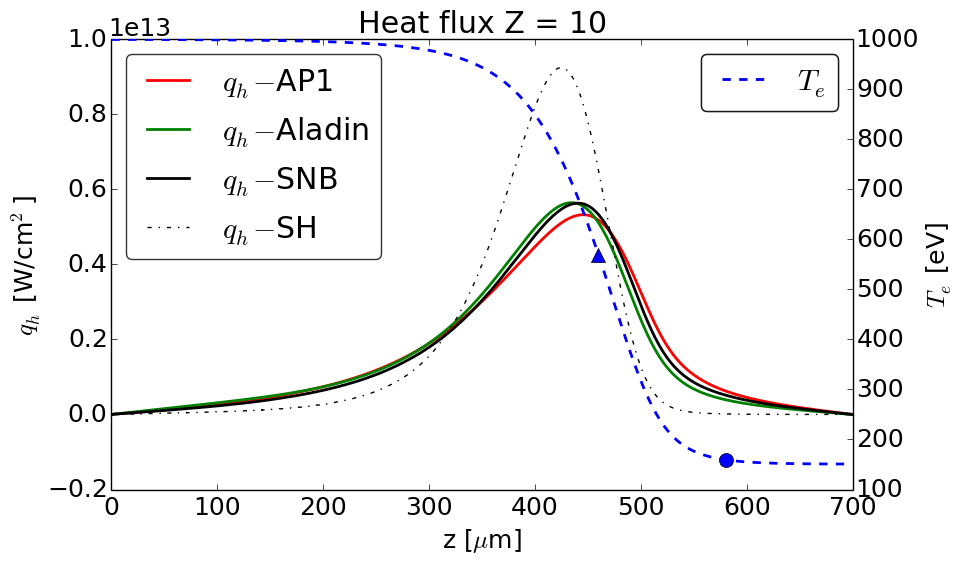
\includegraphics[width=\figscale\textwidth]{../VFPdata/C7_Aladin_case3_heatflux.png} \\
      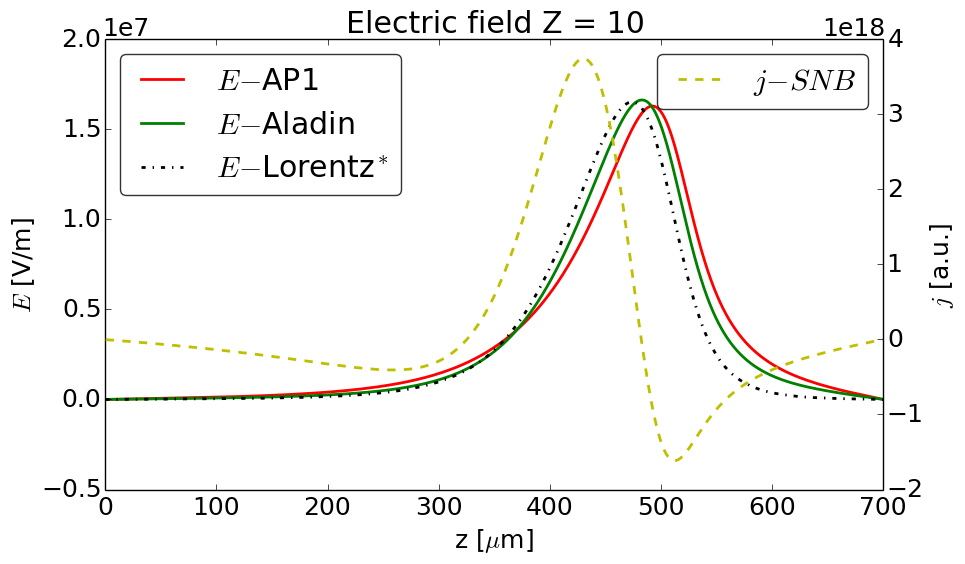
\includegraphics[width=\figscale\textwidth]{../VFPdata/C7_Aladin_case3_Efield.png} \\
      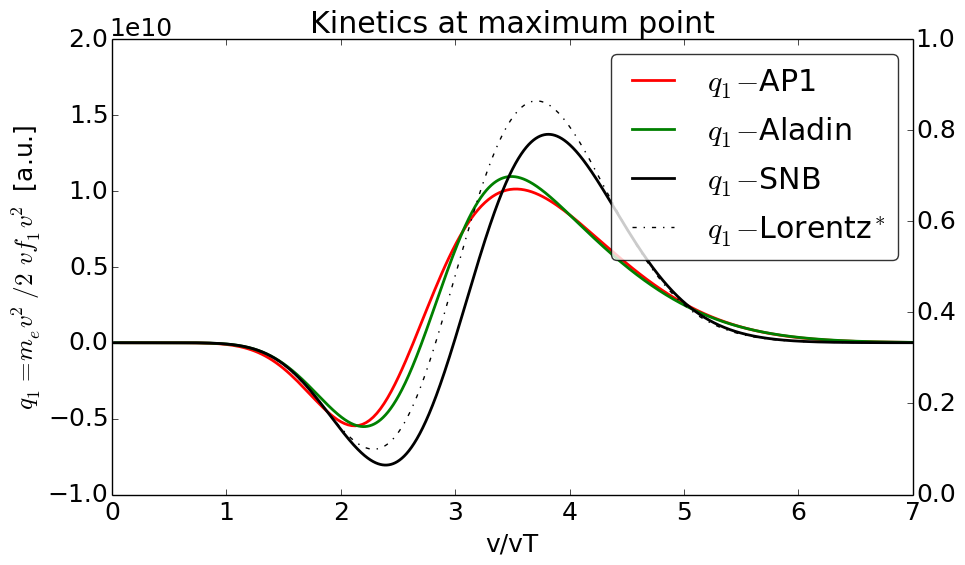
\includegraphics[width=\figscale\textwidth]{../VFPdata/C7_Aladin_case3_kinetics.png} \\
      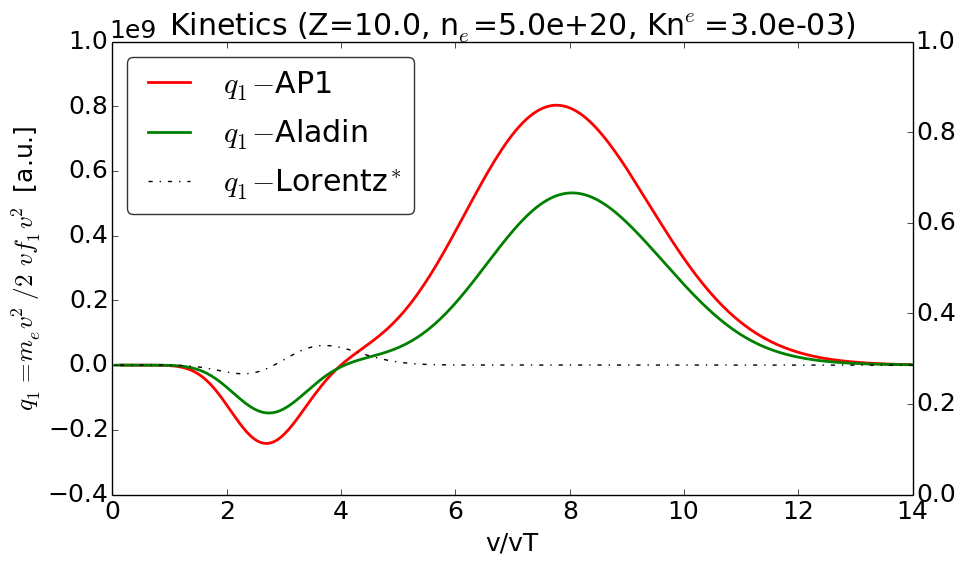
\includegraphics[width=\figscale\textwidth]{../VFPdata/C7_Aladin_case3_nonlocal_kinetics.png}  
    \end{tabular}
  \caption{  
  A~moderate-$\Zbar$ heat-bath problem. The~temperature profile evolved 
  up to 12 ps by Aladin.
  Top plots show heat flux profiles and electric fields by AP1, Aladin, 
  and SNB. The~resulting current of SNB using explicitly the~local electric 
  field $\E_L$ is also shown. Botom plots show a~kinetic detail of
  the~anisotropic part of EDF (its flux velocity moment) at two different 
  spatial points by AP1 and SNB compared to Aladin. 
  %Snapshot 12 ps. Top: correct steady solution of heat flux.  
  %Middle: correct comparison to kinetic profiles at point 460 $\mu$m 
  %by Aladin. 
  %Velocity limit 3.3 $\vth$ at temperature 569.2 eV.
  %Bottom: correct comparison to kinetic profiles at point 580 $\mu$m 
  %by Aladin. Velocity limit 13.1 $\vth$ at temperature 159.4 eV.
  %TODO Fig reordered so change description, E field and current now in Z=10. 
  }
  \label{fig:C7_Aladin_case3}
  \end{center} 
\end{figure}

%Aladin and Impact simulations showed an evolution of the heat flow
%from the local (due to initialising as a Maxwellian) to the
%nonlocal, with a reduced peak, over an initial transient
%phase (over which the temperature ramp flattened somewhat). 
%The transient phase was considered over when the
%ratio of the VFP heat flow to the expected local heat
%flow stopped decreasing. After the transient phase this
%ratio begins to slowly increase as the thermal conduction flattens 
%the temperature ramp and the ratio of the scalelength to mfp increases 
%(i.e. the thermal transport slowly becomes more local). 

The~total computational box size is 700 $\mu$m.
%in the~case of Aladin and Impact and 1000 $\mu$m in the~case of Calder.
We performed Aladin, Impact, and Calder simulations showing an~evolution of
temperature starting from the~initial profile \eqref{eq:T_init}. 
Due to the~initial distribution function being approximated by a~Maxwellian,
the~first phase of the~simulation exhibits a~transient behavior of the~heat
flux. After several ps the~distribution adjusts properly to its asymptotic form
and the~heat flux profiles can be usefully compared. 
We then take the temperature profiles from Aladin/Impact/Calder and compare 
with AP1 and SNB models which calculate a~stationary heat flow
for a~given temperature profile. 
For all heat-bath simulations the electron density, Coulomb logarithm and 
ionisation were kept constant and uniform.
The~Coulomb logarithm was held fixed throughout, $\lnc = 7.09$.

We show AP1 results for two ionization states, namely $\Zbar= 1, 10$ 
in \figref{fig:C7_AladinCalder_case5} and \figref{fig:C7_Aladin_case3}, 
respectively, corresponding to a~moderate nonlocality 
(Kn$^e \sim 10^{-2}$) leading to a~roughly 40 $\%$ inhibition compared 
to the~local SH heat flux maximum. The~original temperature profile steepness
$s = 1/50 \mu$m.
It is preferable to use 
$\text{Kn}^e = \frac{\mfpe}{\sqrt{\Zbar + 1}L_{T_e}}$ instead of
 $\text{Kn} = \frac{\mfpei}{L_{T_e}}$, because $\sqrt{\Zbar + 1}$ provides 
a~better scaling of nonlocality with respect
to ionization \cite{LMV_1983_7}, i.e. the~flux inhibition and Kn$^e$ are
kept approximately the~same when varying $\Zbar$ in 
\figref{fig:C7_AladinCalder_case5} and \figref{fig:C7_Aladin_case3}.
In addition to the~heat flux profiles, we also show the~distribution function 
details related to the~approximate point of the~heat flux maximum (460 $\mu$m) 
and to the~point of the~nonlocal preheat effect (580 $\mu$m) in the~form of
the~flux moment of EDFs anisotropic part \eqref{eq:q1}.
The~nonlocal preheat effect shows a~very good agreement with 
previous results published in \cite{Sherlock_PoP2017}.

The~top left plot of \figref{fig:C7_AladinCalder_case5} shows heat flux 
profiles computed by Aladin, AP1, and SNB corresponding to the~temperature 
$\Te$ profile computed by Aladin and the~top right plot of 
\figref{fig:C7_AladinCalder_case5} shows heat flux profiles computed by Calder, 
AP1, and SNB corresponding to the~temperature $\Te$ profile computed by Calder.
Both kinetic simulations by Aladin and Calder evolved up to 20 ps for 
$\Zbar = 1$. 
The~anisotropic part of EDF, in particular, the~heat flux velocity moment $q_1$, 
at the~heat flux maximum (triangle point) and at~the~nonlocal preheat region 
(circle point) computed by AP1 and SNB for the~temperature profiles by 
Aladin and Calder, can be used as a~detailed comparison of four conceptually
different models: the~full anisotropy form \eqref{eq:LFP_model} of 
the~FP collision operator (Calder); the~isotropic form 
\eqref{eq:C0_collision_operator} of the~FP collision operator (Aladin);
the~simplified linear form \eqref{eq:AWBS_model} of the~FP collision operator
(AWBS in AP1); 
the~nonlocal electron transport model \eqref{eq:SNB_model} (SNB). 
Excellent match of $q_1$ can be seen between 
AP1 and Calder at the~both spatial points. On the~other hand, 
the~AP1 profiles of EDF provide a~reasonable match to Aladin too, however,
one observes a~deviation
%, especially in the~middle plot, 
which resembles to the~low $\Zbar$ trend shown in \figref{fig:q1s_summary}, 
where AP1 corresponds to AWBS and Aladin to BGK curves. To summarize,
various FP-like codes are compared in detail, in particular collisional PIC 
for the first time, and all show a~very good match. 
Furthermore, the~effect of the~anisotropy in the~collision model, 
captured by AP1 and neglected by Aladin and Impact, proves to be important
in the~low-$\Zbar$ plasma. 

In the~case $\Zbar = 10$, we show heat flux profiles
computed by Aladin, AP1, and SNB corresponding to the~temperature $\Te$
profile computed by Aladin up to 12 ps 
in the~top plot of \figref{fig:C7_Aladin_case3}. 
Corresponding profiles of 
a~self-consistently calculated electric fields by Aladin and AP1 
(using the~nonlocal Ohm's law) are shown in the~higher middle plot.
Also the~local theory based electric field $\E_L$ used by SNB is shown.
EDF at the~point of the~approximate heat flux maximum (triangle) of
the~temperature profile is shown in the~lower middle plot, 
where a~very precise match between AP1 and Aladin can be observed, 
and $q_1$ at the~preheat point (circle) of the~temperature profile is shown 
in the~bottom plot. In the~latter case AP1 shows a~very similar properties 
as Aladin with a~difference in magnitude corresponding to a~higher 
heat flux computed by AP1 at this point. 

SNB shows very good results of the~heat flux profile in all three cases, 
i.e. compared to Aladin and Calder in \figref{fig:C7_AladinCalder_case5} 
and to Aladin in \figref{fig:C7_Aladin_case3}. 
However, one can observe that the~EDF kinetic solution of SNB provides 
only a~qualitative image with respect to the~reference green line solution. 
This is illustrated for example in
\figref{fig:C7_Aladin_case3}, where the~kinetics at preheat point plot 
reveals an~insufficient electric field treatment (no return current). 
The~kinetics at maximum point plot shows that the~solution SNB solution
approaches closely the~local Lorentz$^*$ solution and that 
significantly recedes from the~reference fully kinetic solution (green line).
%at the~approximate heat flux maximum
%point in all three cases of $\Zbar$. 
These~discrepancies can be attributed to the~use of an~inconsistent 
electric field in the~case of SNB which uses $\E_L$. An~electric field 
comparison is shown in \figref{fig:C7_Aladin_case3}, where it is shown that 
the~local electric field treatment $\E_L$ used in SNB fails 
in the~preheat region and consequently leads to 
a~significant violation of the~plasma quasi-neutrality,
i.e. a~non-zero current, where one can observe an~uncontrolled stream of 
electrons in the~preheat and also an~overestimation of negative return current
around the~heat flux maximum.

The~AP1 model equations \eqref{eq:AP1f0}, \eqref{eq:AP1f1}, 
and \eqref{eq:AmpereKinetic} in general show a~very good performance 
in all three cases when compared to the~fully kinetic results 
(green line) by Aladin and Calder, which can be assigned 
to the~AWBS collision operator and the~consistent 
treatment of $\E$ via nonlocal Ohm's law \eqref{eq:NonlocalOhm} in
 \eqref{eq:AmpereKinetic} (no $\B$ field in 1D).

In addition, the~Knudsen number Kn$^e$ has been varied among the~simulation 
runs in order to address a~broad range of nonlocality of 
the~electron transport corresponding 
to the~laser-heated plasma conditions, i.e. Kn$^e \in (0.0001, 1)$. 
The~variation of Kn$^e$ arises from the~variation
of the~uniform electron density $n_e \in (10^{19}, 10^{23})$ cm$^{-3}$ or 
the~length scale given by the~slope of the~temperature profile 
$s \in (1/2500, 1/25) \mu$m. Results showing the~heat flux maximum 
of an~extensive set of simulations of
varying Kn$^e$ is shown in \figref{fig:Kn_results}.
 \begin{figure}[htb]
  \begin{center}
    \begin{tabular}{c}
      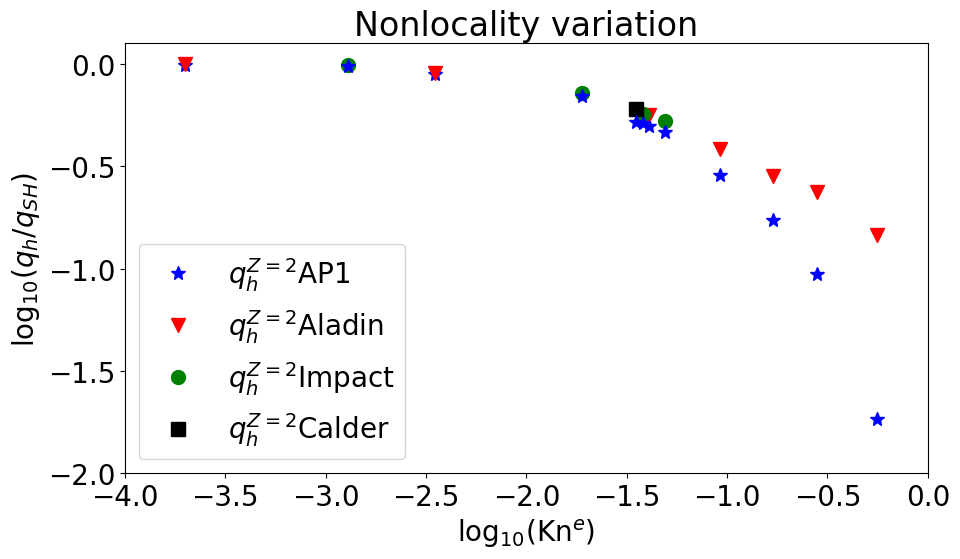
\includegraphics[width=\figscale\textwidth]{Kn_results.png}
    \end{tabular}
  \caption{  
  The~heat-flux inhibition compared to the~local SH theory along varying
  nonlocality (Kn$^e$) in the~heat bath problem. AP1 compares well to 
  the~full kinetic simulations by Aladin, Impact, and Calder, up to 
  Kn$^e \sim 10^{-1}$. For higher nonlocality \textit{decelerating} 
  AP1 departs significanlty from the~reference solutions because of
  the~electric field limiting in accordance with the~velocity limit in 
  \tabref{tab:vlim}. 
  %Simulation results for the case $Z=2$ computed by AP1/Aladin/Impact/Calder.
  %Every point corresponds to the maximum heat flux in a "tanh" temperature 
  %simulation, which can be characterized by Kn. The range of 
  %$\log_{10}(\text{Kn})\in (0, -4)$ can be expressed as equivalent 
  %to the~electron density approximate range n$_e \in (1e19, 3.5e22)$ of 
  %the~50 $\mu$m slope tanh case. In the case of Kn = 0.56, 
  %$q_{Aladin} / q_{AP1}\approx 7.9$.
  }
  \label{fig:Kn_results}
  \end{center} 
\end{figure}
When analyzing the~simulation results shown in \figref{fig:Kn_results}, 
we observed that 
the~maximum of $q_1$ at the~maximum point tends to decrease with increasing 
Kn$^e$ and that the~interval of electron velocities important for 
the~heat transport always belongs to $3 \vth < \vmag <4 \vth$ for an~example
refer to the~kinetics at maximum point in \figref{fig:C7_AladinCalder_case5} 
and \figref{fig:C7_Aladin_case3}. 
We have also found 
an~important observation related to the~electron-electron collisions.
The~stopping force is dominated by
the~electric field for electrons with velocity above the~velocity limit
\begin{equation}
  \vmag_{lim} = \sqrt{\frac{\sqrt{3}\Gamma\me}{2\qe}\frac{n_e}{|\E|}}
  ,
  \label{eq:v_limit}
\end{equation}
as shown in \appref{app:AP1limit} and this limit drops 
down significantly with increasing Knudsen number as can be seen 
in \tabref{tab:vlim}. 
As a~consequence, the~electrons responsible for the~heat flux
($3 \vth < \vmag <4 \vth$) are preferably affected by the~electric field
rather than by collisions when Kn$^{e} > 10^{-1}$. According to 
\tabref{tab:vlim} collsions dominate stopping for $\vmag < 3.1 \vth$ 
when Kn$^e = 10^{-1}$ and even a~much lower value $\vmag < 1.8 \vth$ 
when Kn$^e = 1.0$. This explains the~unsatisfactory results of 
the~\textit{decelerating} AP1
model for high Kn$^e$ shown in \figref{fig:Kn_results}. 
Notably, the~AP1 limited electric field effect (described in 
\appref{app:AP1limit}) leads to a~steep increase of error with respect 
to VFP code Aladin for Kn$^e > 10^{-1}$. 
For example $\vmag_{lim}\sim 4.3\vth$ for the~maximum point EDF in 
\figref{fig:C7_AladinCalder_case5}.

\begin{table}
\begin{center}
  \begin{tabular}{c|ccccc}
    \hline\hline\\
    %Kn$^e$ & $10^{-4}$ & $10^{-3}$ & $10^{-2}$ & $10^{-1}$ & $1$ \\\\
    Kn$^e$ & $\,\,10^{-4}\,\,$ & $\,\,10^{-3}\,\,$ & $\,\,10^{-2}\,\,$ & $\,\,10^{-1}\,\,$ & $\,\,1\,\,$ \\\\
    \hline\\
    $\vmag_{lim} / \vth$ & 70.8 & 22.4 & 7.3 & 3.1 & 1.8\\\\
    \hline\hline
  \end{tabular}
  \caption{
  Scan over varying nonlocality (Kn$^e$) showing the~limit of 
  the~collision friction dominance over the~deceleration of electrons 
  due to the~electric field force. The~electric field effect is dominant
  for electrons with higher velocity than $\vmag_{lim}$ defined in 
  \eqref{eq:v_limit}. Kn$^e$ and $\vth$ are evaluated from the~same 
  plasma profiles.
  %$\sqrt{3}\vmag\frac{\me}{2\qe}\nue > |\E|$.
  }
\label{tab:vlim}
\end{center}
\end{table}

%Yet another observation can be made when analysing the~anisotropic term $q_1$ 
%in \figref{fig:C7_AladinCalder_case5} and \figref{fig:C7_Aladin_case3}. 
%When comparing the~kinetics at maximum and 
%preheat points, both velocity maxima of the~EDF correspond to approximately 
%same electron velocity. This means that the~electrons responsible for 
%the~flux in the~preheat region are those flux dominating electrons 
%from the~maximum point. This provides an~important information
%about the~microscopic motion of electrons on the~nonlocal spatial scale, i.e. 
%a~quantification how far the~fast electrons from the~heat flux maximum 
%are transported before being slowed down significantly. 
%Notice that different reference temperatures and $\vth$ are used 
%in the~maximum and preheat plots, 
%e.g. $\Te = 622$~eV and $\vmag_{q_1^{max}} = 3.24~\vth = 3.39\times10^9$~cm/s 
%at the~maximum point and $\Te = 192$~eV and 
%$\vmag_{q_1^{max}} = 5.95~\vth = 3.46\times10^9$~cm/s at the~preheat point
%in \figref{fig:C7_AladinCalder_case5}.

\begin{comment} % Simulations setup.
In every run of AP1 we used 250~velocity groups in order to avoid
numerical errors in modeling of the~electron kinetics. However, a~smaller 
number of groups, e.g. 50, provides a~very similar results 
(an~error around 10$\%$ in the~heat flux). 
\end{comment} % Simulations setup.

\subsection{Hohlraum problem}
Additionally to the~steep temperature gradients, the~laser-heated plasma 
experiments also involve steep density gradients and variation in ionization,
which is a~dominant effect in multi-material hohlraums
at the interface between the helium gas-fill and 
the ablated high $\Zbar$ plasma.

In~\cite{Brodrick_PoP2017}, a~kinetic simulation of laser pulse interaction 
with a gas filled hohlraum was presented. 
Plasma profiles provided by a~HYDRA simulation in 1D
geometry of a~laser-heated gadolinium hohlraum containing a~helium 
gas at time of 20 ns were used as input for the~IMPACT 
\cite{Kingham_JCP2004} VFP code.  
For simplicity, the Coulomb logarithm was treated as a
constant $\lnc_{ei}$ = $\lnc_{ee}$ = 2.1484. In reality, in the~low-density 
corona $\lnc$ reaches 8, which, however, does not affect the~heat flux profile 
significantly. 
%Plasma profiles at 20 nanoseconds of the~HYDRA simulation 
%were used (after spline smoothing) as the~initial conditions for 
%the~IMPACT run (in planar geometry).
\figref{fig:Gd_VFP_10ps_heatflux} shows the~electron temperature $\Te$ 
evolved during 10 ps by Impact and the~electron density $\ed$ profile
%and ionization $\Zbar$ profiles. 
Along with plasma profiles the~heat flux profiles
of AP1, Impact, and SNB are also shown. 
%\textit{Kn profile will be probably added}. 

\begin{figure}[htb]
  \begin{center}
    \begin{tabular}{c}
      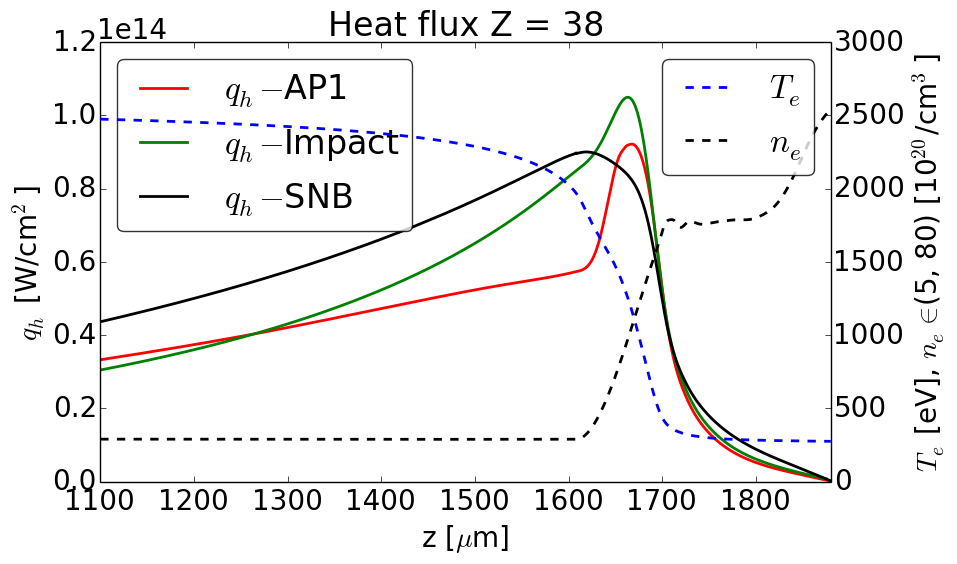
\includegraphics[width=\figscale\textwidth]{../VFPdata/C7_GdHohlraum_heatflux.png}
	  %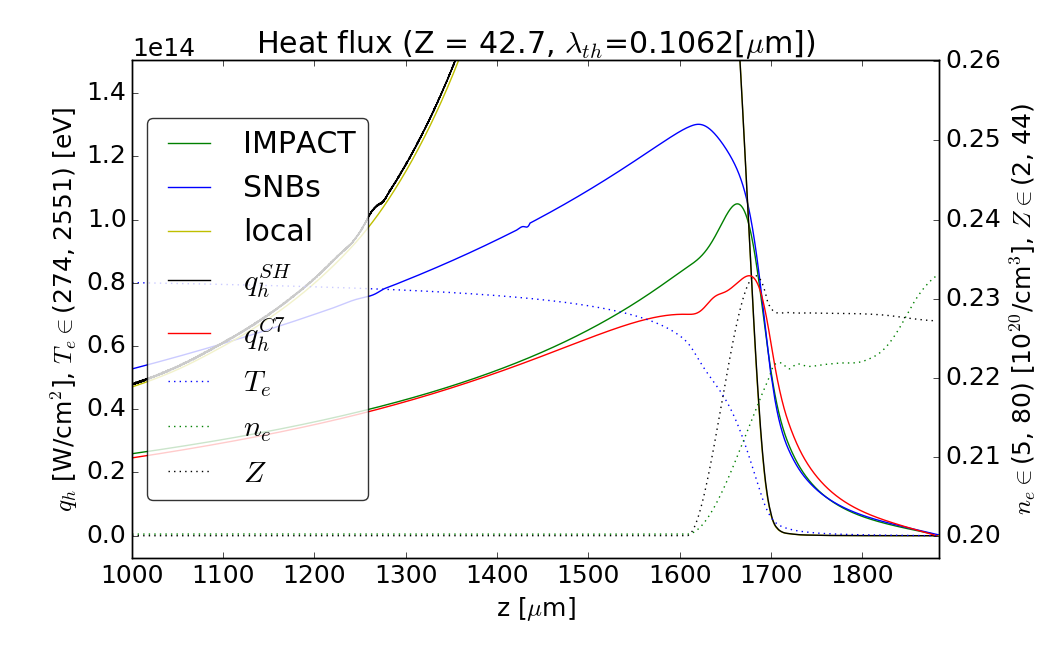
\includegraphics[width=\figscale\textwidth]{../VFPdata/GD_Hohlraum/fluxes_10ps.png} 
    \end{tabular}
  \caption{
  Heat flux profiles by AP1, Impact and SNB along 
  the~electron temperature $\Te$ and electron density $\ed$
  profiles in a~laser-heated gadolinium hohlraum 
  with a~helium gas-fill.
  }
  \label{fig:Gd_VFP_10ps_heatflux}
  \end{center} 
\end{figure}

One can observe a~very good
match between AP1 and Impact computations in the~preheat region.
It is worth mentioning that in the~surroundings of the~heat flux maximum 
($\sim 1662 \mu$m) the~profiles of all plasma variables exhibit steep gradients 
with a change from $T_e$ = 2.5 keV, $n_e$ = 5$\times$10$^{20}$ cm$^{−3}$, 
$\Zbar$ = 2 to $T_e$ = 0.3 keV, $n_e$ = 6$\times$10$^{21}$ cm$^{−3}$ , 
$\Zbar$ = 44 across approximately 100 $\mu$m 
(between 1600~$\mu$m and 1700~$\mu$m), starting at the~helium-gadolinium 
interface.  
In this region, we can see a~qualitative match between AP1 and Impact providing
a~same sign of the~heat flux divergence contributing to hydro, however,
we observe that the~electric field limitation explained in 
\appref{app:AP1limit} leads to a~stronger drop of 
the~\textit{decelerating} AP1 heat flux on the~material 
interface, which then closely aligns to the~Impact heat flux in the~corona. 
On the~other hand, 
SNB overestimates significantly the~heat flux in the~lower density part 
of the~plasma up to the~point of the~heat flux maximum given by Impact 
(green line in \figref{fig:Gd_VFP_10ps_heatflux}), and more 
importantly, the~opposite sign of the~heat flux divergence compared to Impact
(and AP1) in the~steep gradients region close to the~material interface. 
In the~preheat region SNB performs 
very well. Nevertheless, it is important to stress that 
SNB required only 25 velocity groups compared to 250 velocity groups used by
Impact and AP1 for this ICF relevant plasma conditions, thus making it a~very
efficient modeling approach though its description of kinetics is rather
qualitative.
%We also attribute this to the~lack of proper action of the~electric field 
%(the~directional effect) in the~SNB approach.

%
